\documentclass[12pt,a4paper]{article}

% Packages
\usepackage{geometry}
\geometry{margin=1in}
\usepackage{fancyhdr}
\usepackage{titlesec}
\usepackage{listings}
\usepackage{xcolor}
\usepackage{graphicx} 

% Header & Footer
\pagestyle{fancy}
\fancyhf{}
\rhead{DBMS - Assignment 1}
\lhead{Kamithkar Vinod}
\cfoot{\thepage}

% Title formatting
\titleformat{\section}{\large\bfseries}{Problem \thesection:}{0.5em}{}
\titleformat{\subsection}[runin]{\bfseries}{Code:}{0.5em}{}[---]
\titleformat{\subsubsection}[runin]{\bfseries}{Output:}{0.5em}{}[---]

% Code style
\lstset{
    language=cpp,
    basicstyle=\ttfamily\small,
    keywordstyle=\color{blue}\bfseries,
    commentstyle=\color{gray}\itshape,
    stringstyle=\color{red},
    showstringspaces=false,
    numbers=left,
    numberstyle=\tiny\color{gray},
    frame=single,
    breaklines=true
}

% Document Start
\begin{document}

% Title Page
\begin{center}
    \LARGE \textbf{Assignment - 1} \\[0.5cm]
    \Large \textbf{DBMS} \\[1cm]

    \begin{tabular}{rl}
        \textbf{Name:} & Kamithkar Vinod \\
        \textbf{Course:} & PG DAC AUGUST 2025 \\
        \textbf{PRN:} & 250850320040 \\
        \textbf{Form No:} & 250500480 \\
        \textbf{Date:} & 16-10-2025 \\
    \end{tabular}
\end{center}

\vspace{1cm}
\hrule
\vspace{0.5cm}

% Problems
% 1
\section{}
\textbf{Task:} Select all information from Salgrade table.

\subsection{}
\begin{lstlisting}

SELECT * FROM salgrade;

\end{lstlisting}

\subsubsection{}
\begin{center}
    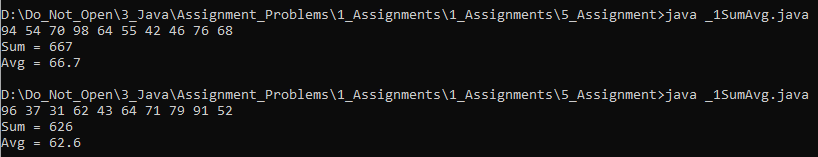
\includegraphics[width=0.8\textwidth]{1.png}
\end{center}


% 2

\section{}
\textbf{Task:} Select all information from emp table.

\subsection{}
\begin{lstlisting}

SELECT * FROM emp;

\end{lstlisting}

\subsubsection{}
\begin{center}
    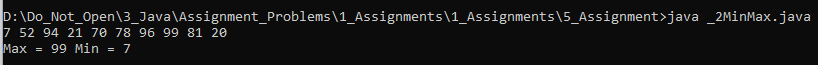
\includegraphics[width=0.8\textwidth]{2.png}
\end{center}

% 3

\section{}
\textbf{Task:} Select all information from dept table.

\subsection{}
\begin{lstlisting}
SELECT * FROM dept;

\end{lstlisting}

\subsubsection{}
\begin{center}
    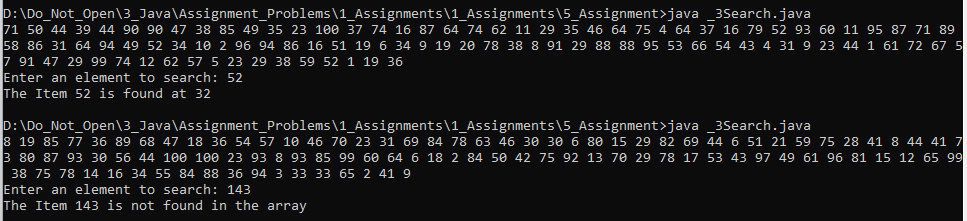
\includegraphics[width=0.8\textwidth]{3.png}
\end{center}

% 4

\section{}
\textbf{Task:} List all employees who have a salary between 1000 and 2000.

\subsection{}
\begin{lstlisting}
SELECT * FROM emp WHERE sal > 1000 AND sal < 2000;

\end{lstlisting}

\subsubsection{}
\begin{center}
    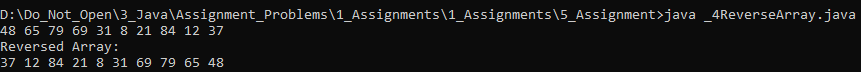
\includegraphics[width=0.8\textwidth]{4.png}
\end{center}

% 5

\section{}
\textbf{Task:} List department numbers and names in department name order.

\subsection{}
\begin{lstlisting}
SELECT * FROM dept ORDER BY dname;

\end{lstlisting}

\subsubsection{}
\begin{center}
    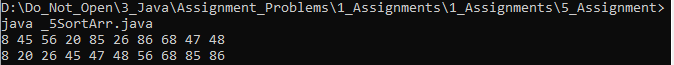
\includegraphics[width=0.8\textwidth]{5.png}
\end{center}

% 6

\section{}
\textbf{Task:} Display all the different job types.

\subsection{}
\begin{lstlisting}
SELECT DISTINCT job FROM emp;;

\end{lstlisting}

\subsubsection{}
\begin{center}
    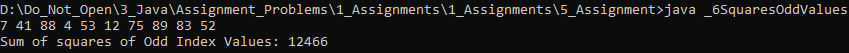
\includegraphics[width=0.8\textwidth]{6.png}
\end{center}

% 7

\section{}
\textbf{Task:} List the details of the employees in departments 10 and 20 in
alphabetical order of employee names.

\subsection{}
\begin{lstlisting}
SELECT FROM WHERE GROUP BY HAVING ORDER BY

SELECT * FROM emp WHERE deptno in (10, 20) ORDER BY ename;

\end{lstlisting}

\subsubsection{}
\begin{center}
    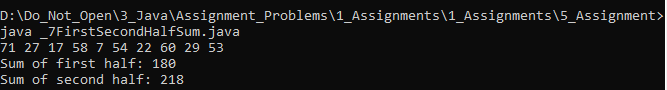
\includegraphics[width=0.8\textwidth]{7.png}
\end{center}

% 8

\section{}
\textbf{Task:} List names and jobs of all clerks in department 20.

\subsection{}
\begin{lstlisting}
SELECT ename, job FROM emp WHERE deptno = 20 AND job = 'CLERK';

\end{lstlisting}

\subsubsection{}
\begin{center}
    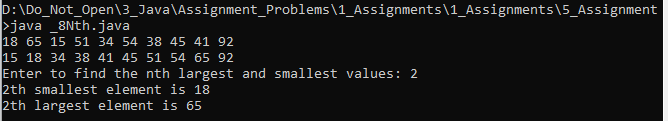
\includegraphics[width=0.8\textwidth]{8.png}
\end{center}

% 9

\section{}
\textbf{Task:} Display all employee names which have TH or LL in them.

\subsection{}
\begin{lstlisting}
SELECT ename FROM emp WHERE ename LIKE '%TH%' OR ename LIKE '%LL%';

SELECT ename FROM emp WHERE ename REGEXP 'TH|LL';

\end{lstlisting}

\subsubsection{}
\begin{center}
    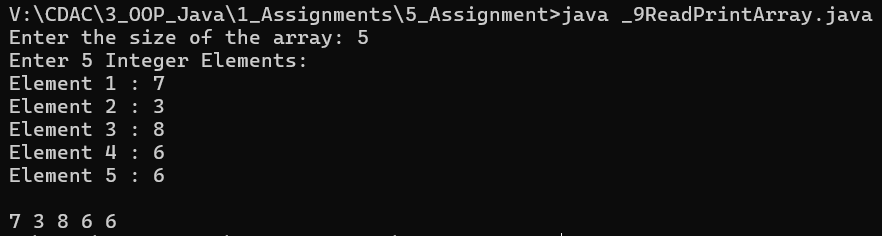
\includegraphics[width=0.8\textwidth]{9.png}
\end{center}

% 10

\section{}
\textbf{Task:} List the details of the employees who have a manager.

\subsection{}
\begin{lstlisting}
SELECT * FROM emp WHERE job = 'manager';

\end{lstlisting}

\subsubsection{}
\begin{center}
    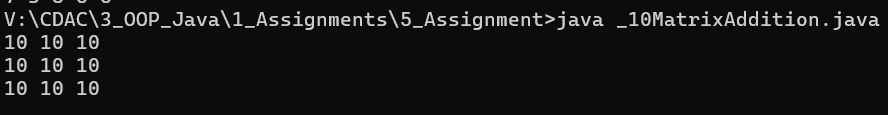
\includegraphics[width=0.8\textwidth]{10.png}
\end{center}

% 11

\section{}
\textbf{Task:} Display the name and the total remuneration for all employees.

\subsection{}
\begin{lstlisting}
SELECT ename, (ifnull(comm, 0) + sal) "Total Remuneration" FROM emp;

\end{lstlisting}

\subsubsection{}
\begin{center}
    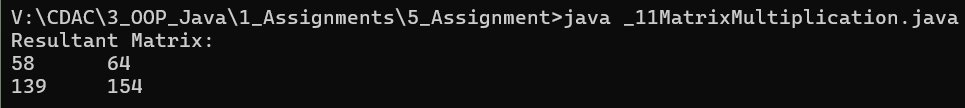
\includegraphics[width=0.8\textwidth]{11.png}
\end{center}

% 12

\section{}
\textbf{Task:} Display name, annual salary and commission of all sales people
whose monthly salary is greater than their commission. The output
should be ordered by salary highest first. If two or more employees
have the same salary sort by employee name, within the highest
salary order.

\subsection{}
\begin{lstlisting}
SELECT ename, sal, comm FROM emp 
WHERE sal > ifnull(comm, 0) AND job = 'SALESMAN'
ORDER BY sal DESC, ename ASC;

\end{lstlisting}

\subsubsection{}
\begin{center}
    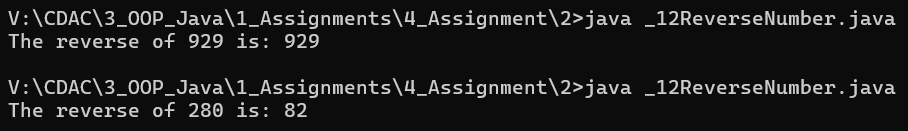
\includegraphics[width=0.8\textwidth]{12.png}
\end{center}

% 13

\section{}
\textbf{Task:} Display all employees who were hired during 1982.

\subsection{}
\begin{lstlisting}
SELECT * FROM emp WHERE year(hiredate) = 1982;

\end{lstlisting}

\subsubsection{}
\begin{center}
    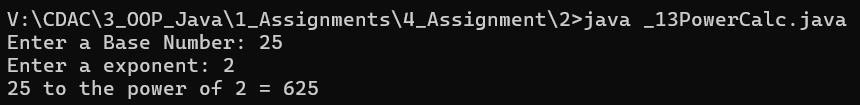
\includegraphics[width=0.8\textwidth]{13.png}
\end{center}

% 14

\section{}
\textbf{Task:} Display the employee name and job by concatenating them and
give an appropriate heading.

\subsection{}
\begin{lstlisting}
SELECT concat(ename, ' is a ', job) "Employee Details" FROM emp;

\end{lstlisting}

\subsubsection{}
\begin{center}
    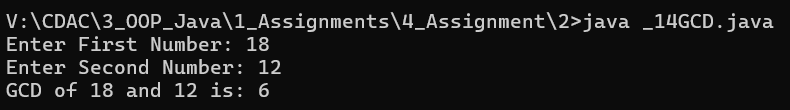
\includegraphics[width=0.8\textwidth]{14.png}
\end{center}

% 15

\section{}
\textbf{Task:} Display the employee name and the job in brackets.

\subsection{}
\begin{lstlisting}
SELECT concat(ename, ' [', job, ']') "Employee Details" FROM emp;

\end{lstlisting}

\subsubsection{}
\begin{center}
    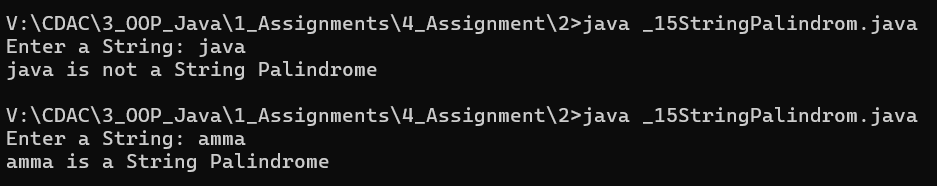
\includegraphics[width=0.8\textwidth]{15.png}
\end{center}

% 16

\section{}
\textbf{Task:} It has been discovered that the sales people in department 30 are
not all male. Hence display the job of salesman as salesperson.

\subsection{}
\begin{lstlisting}
SELECT REPLACE(job, 'SALESMAN', 'SALESPERSON') FROM emp;

SELECT
    empno,
    ename,
    CASE
        WHEN job = 'SALESMAN' AND deptno = 30 THEN 'SALESPERSON'
        ELSE job
    END AS job,
    mgr,
    hiredate,
    sal,
    comm,
    deptno
FROM
    emp;

\end{lstlisting}

\subsubsection{}
\begin{center}
    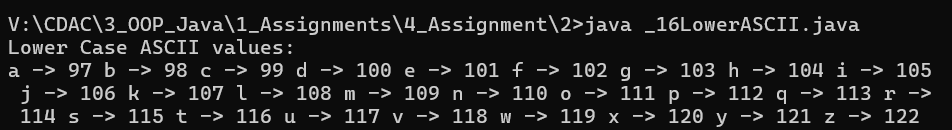
\includegraphics[width=0.8\textwidth]{16.png}
\end{center}


\end{document}



